\section{Unterschiedliche Charakter}
Spiele verwenden die unterschiedlichsten Charaktere, nicht nur das Aussehen sondern auch die Komplexität der Körperteile und die Anzahl der Knochen variiert. Um den Charaktercontroller vielseitig einsetzbar zu gestalten wird in diesem Kapitel die Walker Demo Komponenten angepasst um den Einrichtungsprozess zu vereinfachen und unterschiedliche Charakter Körperstrukturen zu erlauben. Es wird analysiert wie das Agentenskript angepasst werden muss um Charaktere mit unterschiedlichen Körperstrukturen zu steuern und zu trainieren. Anschließend wird der Einrichtungsprozess am Beispiel eines Mixamo 3D Charakter Modells dargestellt. Zum Schluss wird der Mixamo Charakter trainiert und das Ergebnis ausgewertet.

\subsection{Anforderungen}	
Der Agent der Walker Demo setzt für jedes Körperteil eine separate Referenz, die über den Inspector in Unity konfiguriert werden muss. Um die damit verbundene Einschränkung einer festgelegten Konfiguration von Körperteilen zu beheben, soll eine flexible Liste von Körperteilen konfiguriert werden. Bei der Zustandserfassung der Körperteile soll anschließend der Zustand aller Körperteile in der Liste erfasst werden. Die Aktion soll gleichermaßen Zielwinkel und Gelenkstärke für alle Körperteile der Liste beinhalten. Um unnötige Komplexität bei der Beobachtung und Aktion zu vermeiden, sollen die Zielwinkel nur für bewegbare Gelenkachsen bestimmt werden. Die Gelenkstärke soll für komplett versteifte Gelenke ebenfalls ausgelassen werden. Um die Konfiguration weiter zu erleichtern, sollen die Körperteile zudem automatisch dem Walker-Agenten hinzugefügt werden. Schließlich soll auch das \hl{Stabilisierungsobjekt} automatisch generiert werden.

\subsection{Anpassungen}
Um ein Objekt als Körperteil zu definieren, wurde die Bodypart-Klasse in ein MonoBehaviour-Unity-Skript umgewandelt. Zusätzlich wurden die Funktionen zur Steuerung der Körperteile von der Gelenk-Motor-Steuerung in das Körperteil-Skript verlagert. Dadurch ist es möglich, die Körperteile direkt über das Körperteil-Skript zu steuern, ohne den Umweg über die Gelenk-Motor-Steuerung. Die Körperteilkomponente initialisiert sich beim Programmstart und ist anschließend sowohl für die Steuerung als auch für die Aktualisierung der Zustandsparameter des Körperteils zuständig. Jedes Körperteil benötigt eine Festkörperkomponente. Zusätzlich wird überprüft, ob das Objekt über eine Gelenkkomponente verfügt. Existiert eine solche Komponente, wird diese eingerichtet und die Freiheitsgrade bestimmt. Diese Freiheitsgrade geben an, welche Felder für das Körperteil in der Beobachtung und Aktion hinzugefügt werden müssen.

Der Walker-Agent sucht beim Programmstart alle Körperteile und speichert sie in einer Liste ab. Beim Erstellen der Beobachtung und beim Umwandeln der Aktion in eine Bewegung wird über die Körperteilliste iteriert, und für jedes Körperteil wird die entsprechende Beobachtung erstellt oder die Aktion ausgeführt.
Das \hl{Stabilisierungsobjekt} wird auch automatisch beim initialisieren des Agenten erstellt (siehe \ref{lst:walker_agent_angepasst}).

\begin{lstlisting}[caption={Ausschnitt Angepasstes Walker Agent Skript},captionpos=b,label={lst:walker_agent_angepasst}]
public override void Initialize()
{
    //Stabilisierungs- / Orientierungsobjekt erstellen
    GameObject orientationObject = new GameObject("OrientationObject");
    orientationObject.transform.parent = transform;
    walkOrientationCube = orientationObject.AddComponent<OrientationCubeController1>();
    walkOrientationCube.root = root;
    walkOrientationCube.target = target;

    //Körperteile initialisieren und zur Liste hinzufügen
    foreach (Bodypart bps in root.GetComponentsInChildren<Bodypart>())
    {
        bps.Initialize();
        bps.onTouchingGround.AddListener(OnTouchingGround);
        bp.onTouchedTarget.AddListener(OnTouchedTarget);
        bodyparts.Add(bps);
    }
}

//Körperteile zurücksetzen
public override void OnEpisodeBegin()
{
    foreach (Bodypart bps in bodyparts)
    {
        bps.Reset();
    }
}

//Beobachtung für Körperteil hinzufügen
public void CollectObservationBodyPart(Bodypart bps, VectorSensor sensor)
{
    sensor.AddObservation(bps.touchingGround);

    sensor.AddObservation(m_OrientationCube.transform
    .InverseTransformDirection(bps.rb.velocity));
    sensor.AddObservation(m_OrientationCube.transform
    .InverseTransformDirection(bps.rb.angularVelocity));

    sensor.AddObservation(m_OrientationCube.transform
    .InverseTransformDirection(bps.rb.position - root.position));

    if (bps.dof.sqrMagnitude <= 0) return;

    sensor.AddObservation(bps.rb.transform.localRotation);
    sensor.AddObservation(bps.currentStrength / bps.physicsConfig.maxJointForceLimit);

}

//Körperteilbeobachtungen an Beobachtung anfügen
public override void CollectObservations(VectorSensor sensor)
{
foreach (Bodypart bps in bodyparts)
    {
        CollectObservationBodyPart(bps, sensor);
    }
}

//Aktion in Bewegung umwandeln
public override void OnActionReceived(ActionBuffers actionBuffers)
{
    var continuousActions = actionBuffers.ContinuousActions;
    int i = -1;

    foreach (Bodypart bp in bodyparts)
    {
        if (bp.dof.sqrMagnitude <= 0) continue;
        float targetRotX = bp.dof.x == 1 ? continuousActions[++i] : 0;
        float targetRotY = bp.dof.y == 1 ? continuousActions[++i] : 0;
        float targetRotZ = bp.dof.z == 1 ? continuousActions[++i] : 0;
        float jointStrength = continuousActions[++i];
        bp.SetJointTargetRotation(targetRotX, targetRotY, targetRotZ);
        bp.SetJointStrength(jointStrength);
    }
}
\end{lstlisting}


\subsection{Einrichtung}
Der ausgewählte Charakter ist der Y Bot Charakter welcher in Abbildung \ref{fig:charakter_mixamo} zu sehen ist. Der Y Bot besteht ausgenommen der Finger aus 22 Knochen. Um das Training zu beschleunigen werden für alle Versuche die Finger mit dem Handknochen als ein Körperteil zusammengefasst.

\begin{figure}[H]
  \centering  
  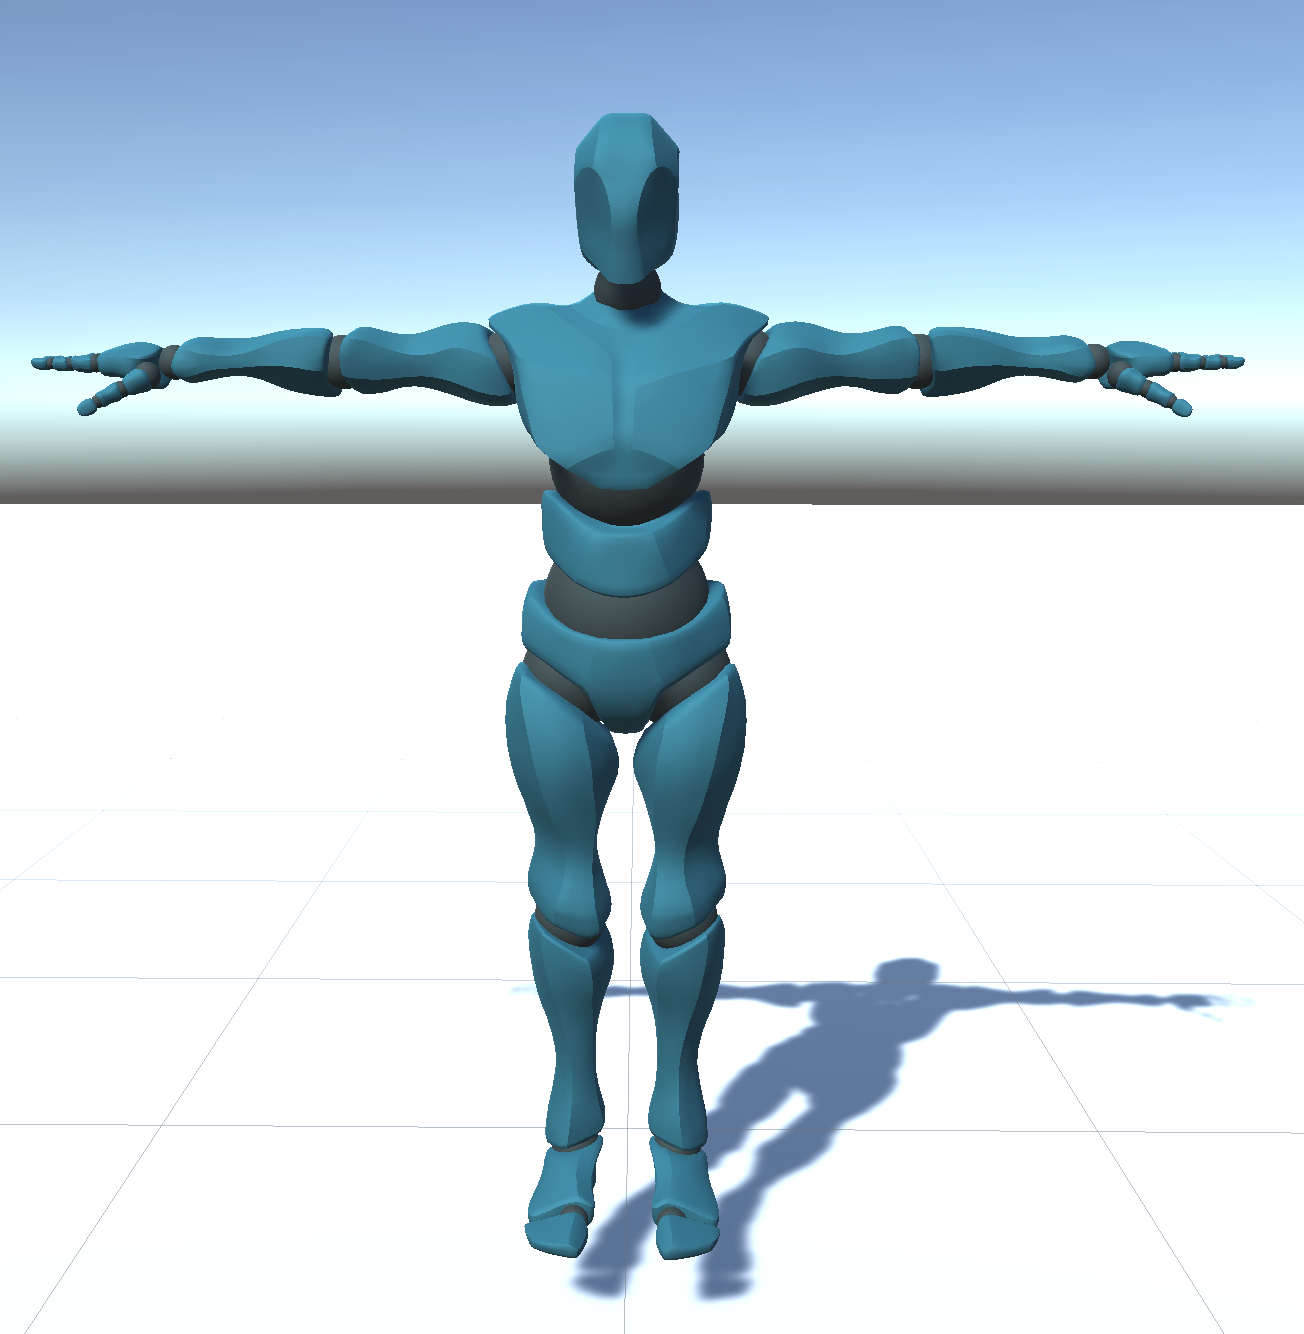
\includegraphics[scale=0.5]{img/charakter_mixamo}
  \caption{Mixamo Charakter Y Bot}
  \label{fig:charakter_mixamo}
\end{figure}

Jedes Körperteil benötigt für das Steuern und Trainieren mit dem Walker Agenten Skript eine Kollisionskomponente, eine Festkörperkomponente und eine Körperteilkomponente. Zusätzlich müssen Gelenkkomponenten hinzugefügt werden, um die Körperteile miteinander zu verbinden. Dabei wird die Gelenkkomponente jeweils auf das untergeordnete Körperteil angewendet, während das übergeordnete Körperteil als verbundener Körper referenziert wird. Die Kollisionskomponente soll das Körperteil in vereinfachter Form und Größe darstellen, um die Berechnungen zu optimieren. Bei den Festkörpern müssen das Gewicht und der Schwerpunkt festgelegt werden, um eine realistische physikalische Simulation zu gewährleisten. In der Gelenkkomponente können Bewegungen durch das Festlegen von Winkellimits gesperrt oder limitiert werden. Für die Rotationsberechnung wird der Slerp-Modus verwendet, da dieser eine gleichmäßige Interpolation der Rotation ermöglicht. In der Körperteilkomponente können Parameter wie Stärke und maximale Rotationsgeschwindigkeit angepasst werden, wobei die Standardwerte aus der Walker Demo in den meisten Fällen ausreichend sind. Bei Bedarf kann auch das Feld "Trigger Touching Ground" aktiviert werden, um ein Event auszulösen, sobald das Körperteil den Boden berührt.

\begin{figure}[H]
  \centering  
  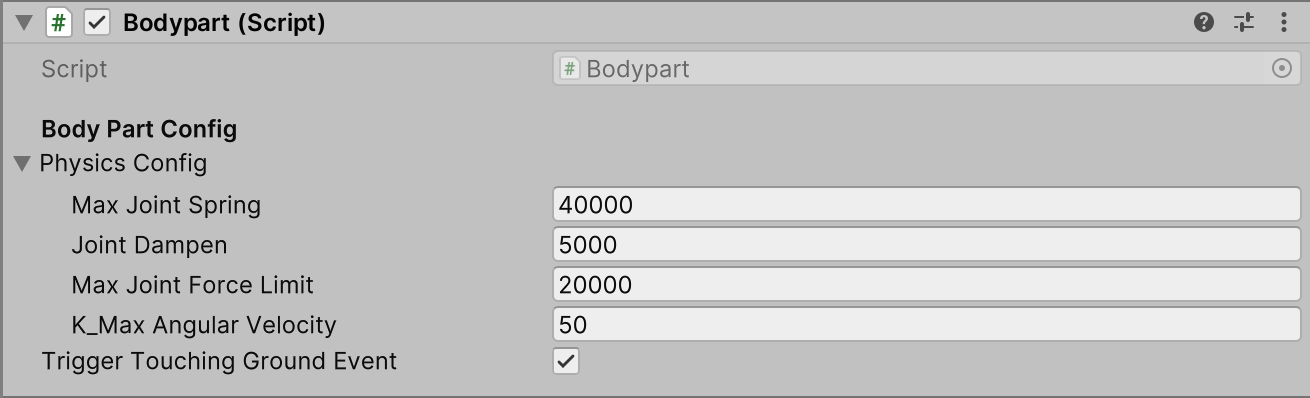
\includegraphics[scale=0.5]{img/komponente_bodypart}
  \caption{Körperteilkomponente}
  \label{fig:komponente_bodypart}
\end{figure}


Ist der Körper fertig konfiguriert wird zuletzt das Walker Agent Skript und der Decision Requester hinzugefügt.

\begin{figure}[H]
  \centering  
  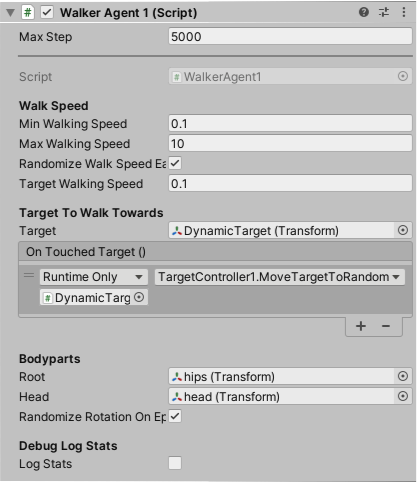
\includegraphics[scale=0.5]{img/komponente_agent_walker1}
  \caption{Walker Agentkomponente}
  \label{fig:komponente_agent_walker1}
\end{figure}

Die Gewichte der Körperteile wurden von der Walker Demo übernommen. Gleichermaßen wurden die Winkellimits für die Gelenke übernommen. Die zusätzlichen Körperteile wurden vereinfacht. Der Oberkörper besteht im Mixamo Modell aus den Schulterknochen sowie dem obersten Wirbel der Wirbelsäule. Die Wirbelsäule besteht im Mixamo Modell aus 2 Wirbeln anstatt dem einen Wirbel des Läufers aus der Demo. Zuletzt sind die Füße noch in Fuß und Vorderfuß aufgeteilt. Bei diesen Änderungen der Körperstruktur wurden die Gewichte und Winkellimits des vereinfachten Körpers auf die komplexeren Körperstrukturen aufgeteilt.

\begin{table}[H]
  \centering
  {\rowcolors{1}{gray!10}{white}
  \begin{tabular}{ |p{3cm}|p{3cm}|p{2cm}|p{4cm}|p{2cm}| }
  \hline
  \textbf{Körpertei}l& \textbf{Verbundenes Körperteil} & \textbf{Gewicht} & \textbf{Winkellimits} & \textbf{Form} \\
  \hline
  Hüfte & - & 15kg & - & Kapsel \\
  \hline
  Wirbel 1 & Hüfte & 6kg & x(-20,20) y(-20,20) z(-15,15) & Kugel \\
  \hline
  Wirbel 2 & Wirbel 1 & 4kg & - & Kugel \\
  \hline
  Wirbel 3 & Wirbel 2 & 3kg & x(-20,20) y(-20,20) z(-15,15) & Kugel \\
  \hline
  Schulter LR & Wirbel 3 & je 2kg& - & Kugel \\
  \hline
  Nacken & Wirbel 3 & 1kg & - & Kugel \\
  \hline
  Kopf & Nacken & 6kg & x(-30,10) y(-20,20) & Kapsel \\
  \hline
  Oberarm LR & Oberkörper & je 4kg & x(-60,120) y(-100,100) & Kapsel \\
  \hline
  Unterarm LR & Oberarm & je 3kg & x(0,160) & Kapsel \\
  \hline
  Hand LR & Unterarm & je 2kg & - & Quader \\
  \hline
  Oberschenkel LR & Hüfte & je 14kg& x(-90,60) y(-40,40) & Kapsel \\
  \hline
  Unterschenkel LR & Oberschenkel & je 7kg &  x(0,120) & Kapsel \\
  \hline
  Fuß LR & Unterschenkel & je 4kg & x(-20,20) y(-20,20) z(-20,20) & Quader \\
  \hline
  Vorderfuß LR & Fuß & je 1kg & - & Quader \\
  \hline
  \end{tabular}}
  \caption{Mixamo Charakter Körperteile}
  \label{table:mixamo_körperteile}
\end{table}

\subsection{Auswertung}
Das Training dauert etwa doppelt so lange um ein ähnliches Resultat zu erreichen. Der Agent lernt mit dem Mixamo Modell lange in der Umgebung zu bestehen und erreicht dabei auch ein gutes Maß an Belohnung pro Schritt (siehe Graphen). In der Abbildung \ref{fig:mixamo_versuch10_gangbild} wird das erlernte Gangbild gezeigt. Der Läufer lernt in diesem Fall nicht das Laufen sondern galoppiert zum Ziel.

\hl{106 Tensorboard Graphen einfügen}

\begin{figure}[H]
  \centering
  \begin{tabular}{cccc}
    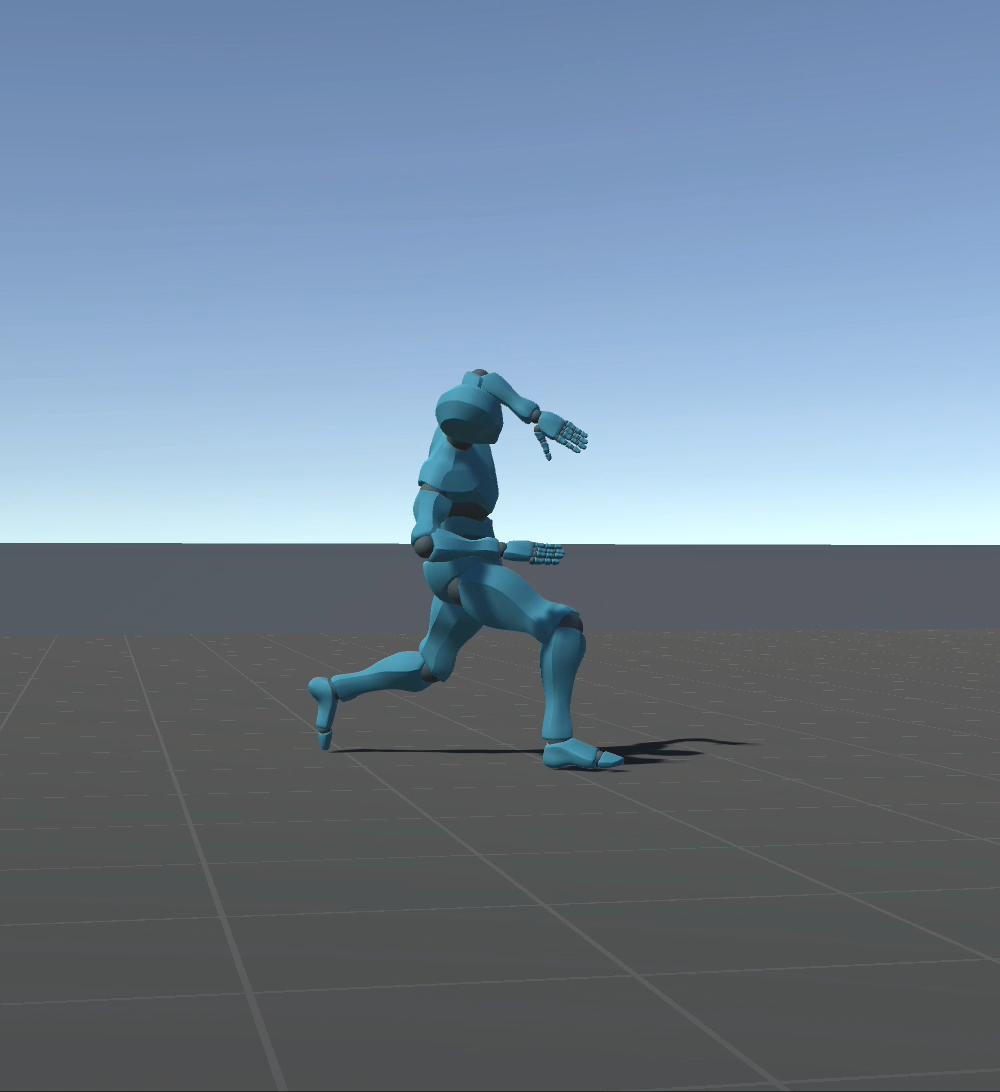
\includegraphics[width=0.2\textwidth]{img/charakter_mixamo_galoppieren1} & 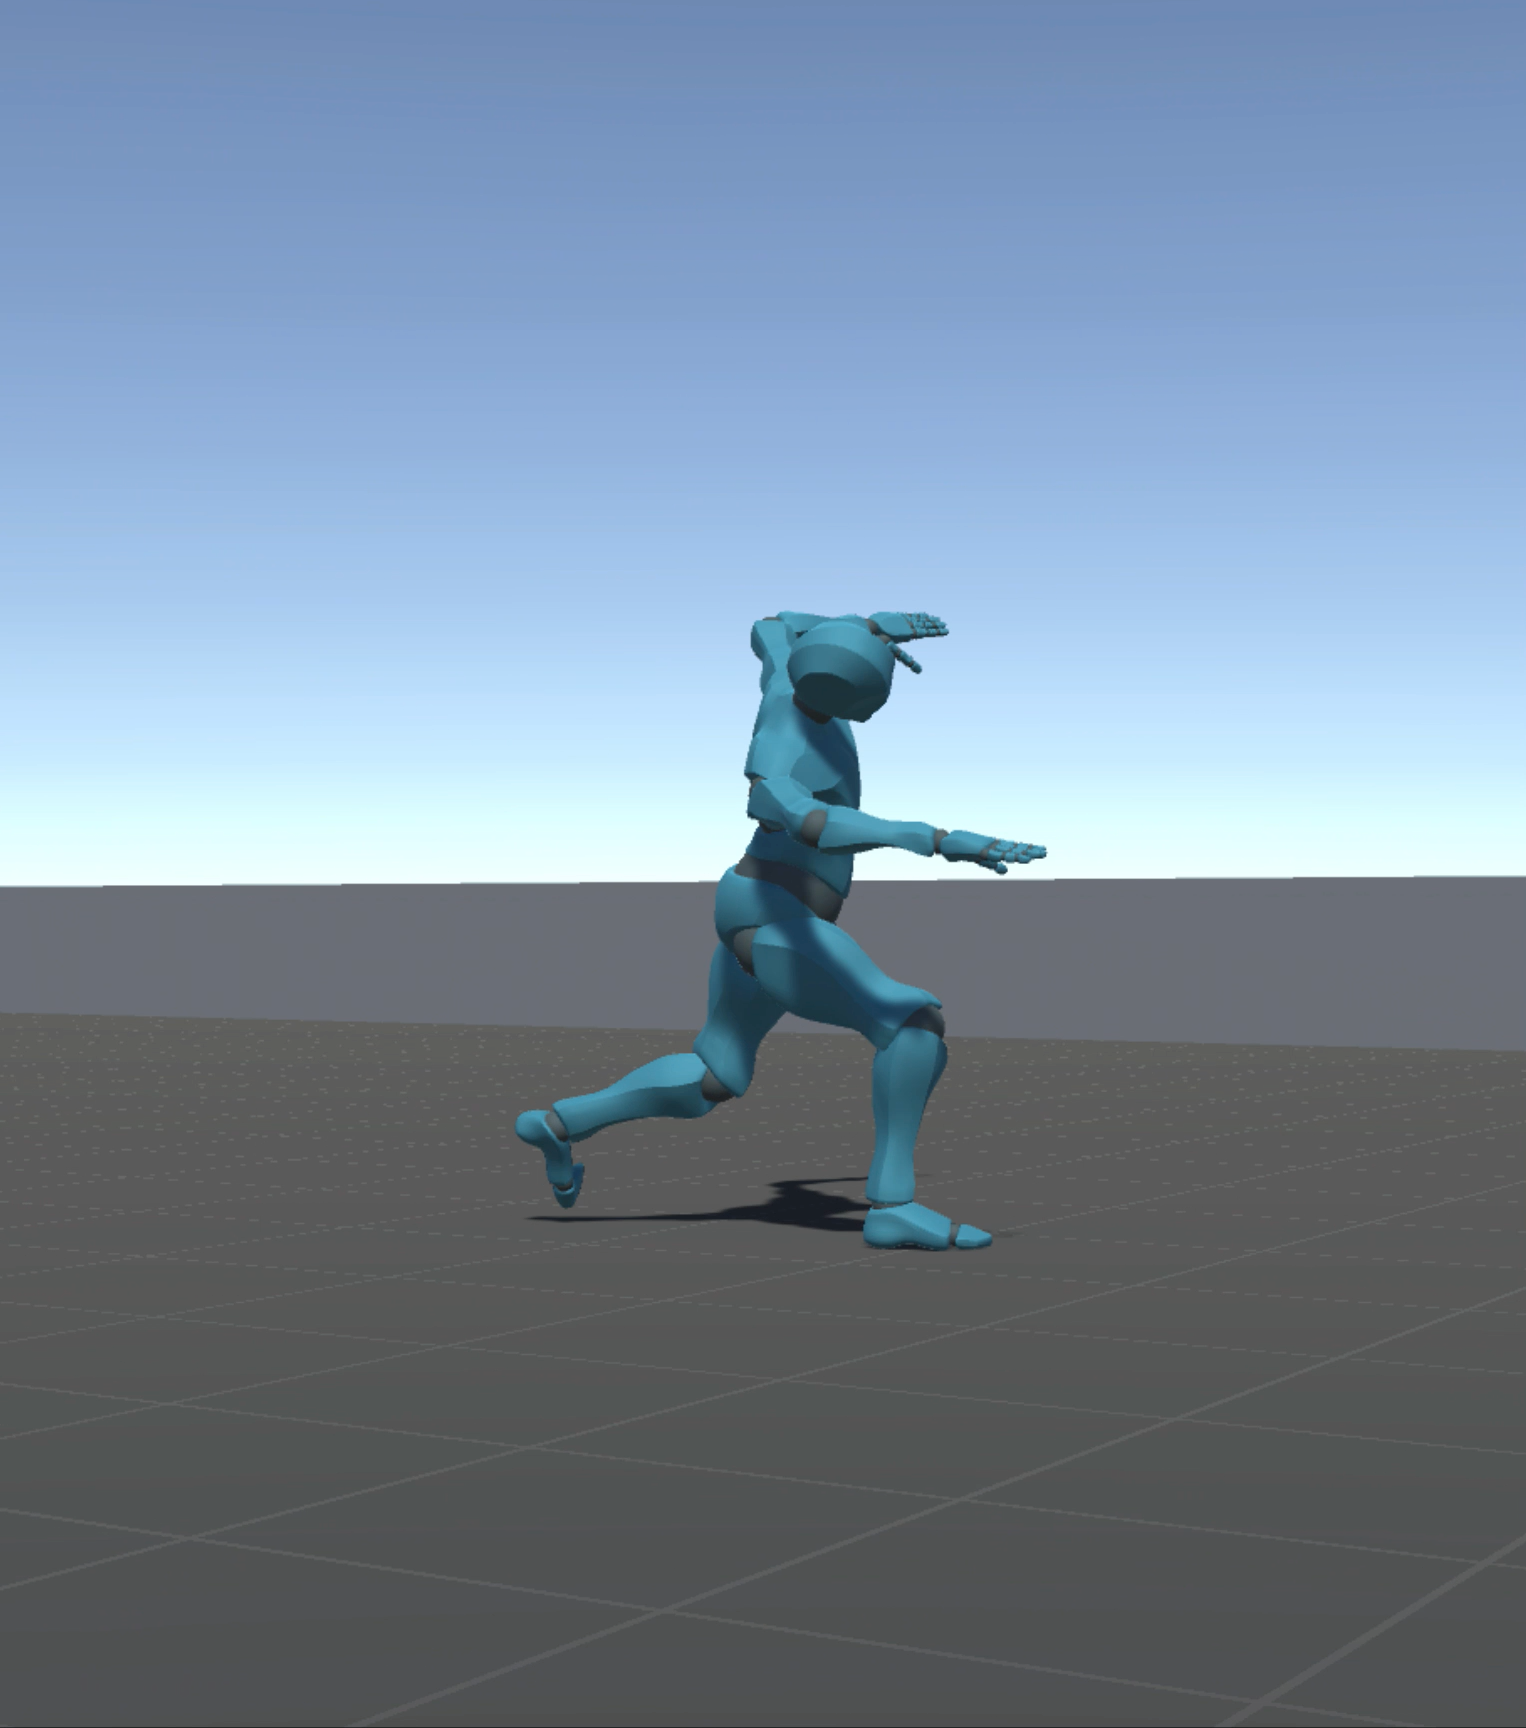
\includegraphics[width=0.2\textwidth]{img/charakter_mixamo_galoppieren2} & 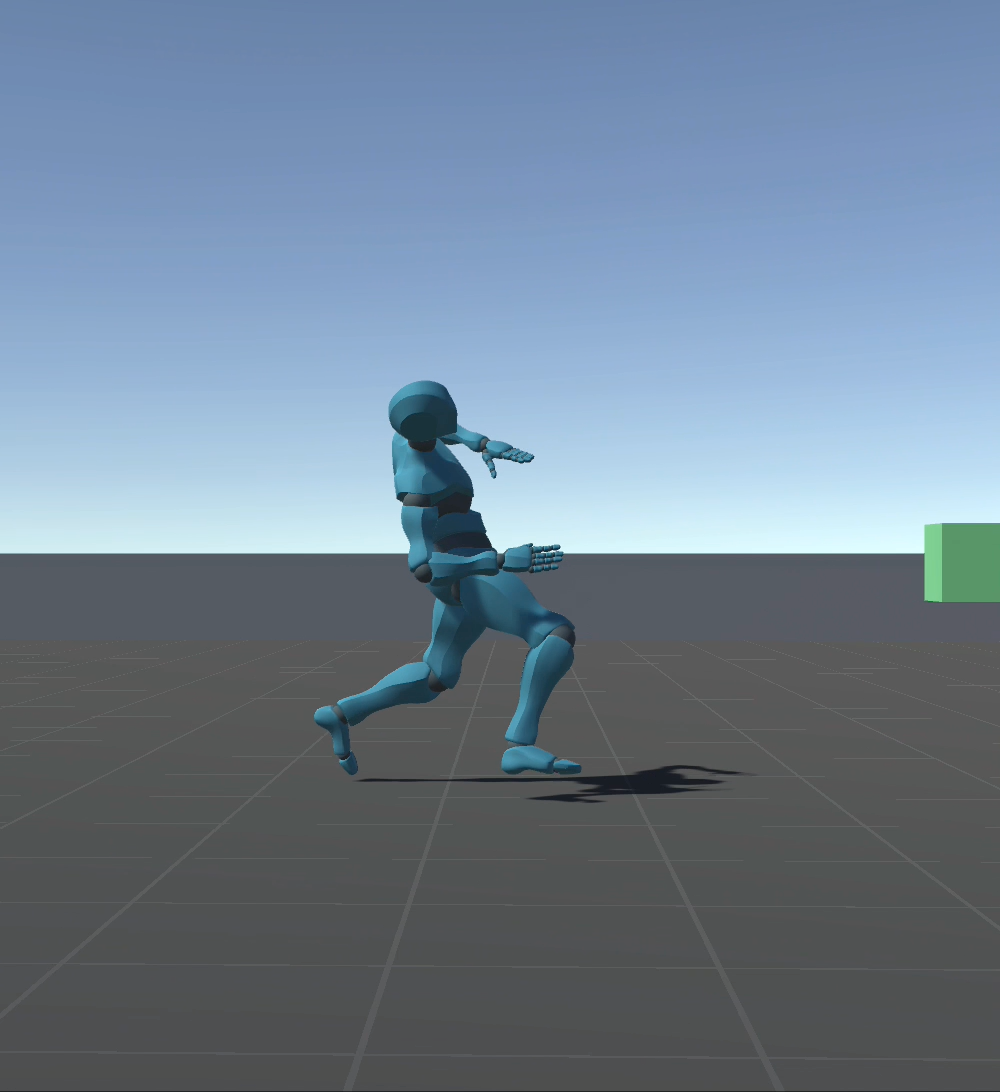
\includegraphics[width=0.2\textwidth]{img/charakter_mixamo_galoppieren3} & 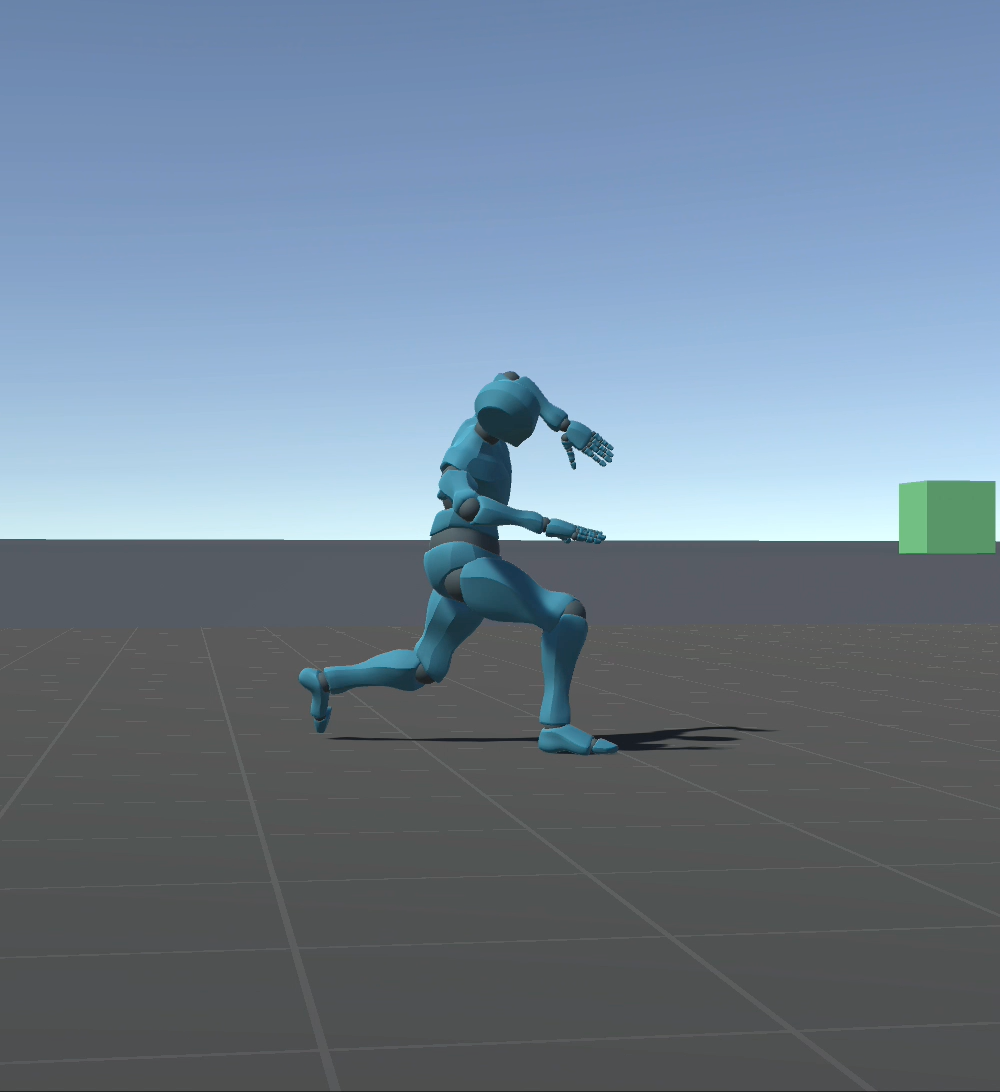
\includegraphics[width=0.2\textwidth]{img/charakter_mixamo_galoppieren4} \\
  \end{tabular}
  \caption{Mixamo Versuch 10 Gangbild}
  \label{fig:mixamo_versuch10_gangbild}
\end{figure}